%%\documentclass[12pt,oneside,a4paper]{article}
%\documentclass[11pt,oneside]{amsart}
%\usepackage{amsmath,amssymb,amsfonts}
%%\usepackage{algorithmic}
%\usepackage{graphicx}
%%\usepackage{textcomp}
%%\usepackage{xcolor}
%%\usepackage{pdfpages}
%%\def\BibTeX{{\rm B\kern-.05em{\sc i\kern-.025em b}\kern-.08em
%%    T\kern-.1667em\lower.7ex\hbox{E}\kern-.125emX}}
%
%\usepackage{amscd}
%%\usepackage[section]{placeins}
%%\usepackage{float}
%%\usepackage[T2A,T1]{fontenc}
%%\usepackage{array}
%\usepackage[utf8]{inputenc}
%\usepackage[english]{babel}
%\usepackage{enumitem}
%\usepackage{graphicx}
%\usepackage[hidelinks]{hyperref}
%\usepackage{caption}
%%\usepackage{epstopdf}
%\usepackage{url}
%\usepackage[numbers,sort&compress]{natbib}
%
%
%\usepackage{mathtools}
%%\usepackage{cuted}
%%\usepackage{flushend}\usepackage{amsmath}
%%\usepackage{amsfonts}
%%\usepackage{amssymb}
%%\hypersetup{draft}



%\usepackage{todonotes}
%
%%\setlength{\topmargin}{-1.5cm}
%%\setlength{\textheight}{24cm}
%%\setlength{\oddsidemargin}{0cm}
%%\setlength{\textwidth}{16cm}
%
%%\usepackage{showframe}% <-- only for show page layout, in real document had to be deleted
%%\renewcommand*\ShowFrameColor{\color{red}}
%
%%\usepackage{tcolorbox}
%%\newtcolorbox{mybox}{colback=red!5!white,colframe=red!75!black}
%
%
%%
%
%%\usepackage[version=4]{mhchem}
%
%%\renewcommand{\figurename}{Fig.}
%%\usepackage[figurename=Fig.]{caption}
%%\newcommand{\eqnref}[1]{(\ref{#1})}
%
%\usepackage{subfig}
%
%\usepackage{setspace}
%\usepackage{todonotes}
%
%
%\usepackage[normalem]{ulem}
%\usepackage[nomargin,inline,marginclue,draft]{fixme}
% \fxsetup{theme=color, mode=multiuser} 
% \FXRegisterAuthor{pb}{apb}{\color{blue}PB} 
% \FXRegisterAuthor{va}{ava}{\color{red}VA} 
% \FXRegisterAuthor{bmb}{abmb}{\color{yellow}BMB} 
% \newcommand{\FXUser}[2]{\todo[inline,size=\small]{{\bfseries #1:} #2}}

%\documentclass[11pt]{amsart}
\documentclass[3p,review,authoryear]{elsarticle}
\DeclareUnicodeCharacter{0308}{\forall}
\usepackage{geometry}                % See geometry.pdf to learn the layout options. There are lots.
\geometry{a4paper}                   % ... or a4paper or a5paper or ... 
%\geometry{landscape}                % Activate for for rotated page geometry
%\usepackage[parfill]{parskip}    % Activate to begin paragraphs with an empty line rather than an indent
\usepackage{graphicx}
\usepackage{natbib}
\usepackage{adjustbox}
\usepackage{amssymb}
\usepackage{rotating}
\usepackage{hyperref}
\usepackage{booktabs}
\usepackage{subfig}
\usepackage{engord}
%\usepackage{amsaddr}
\usepackage{url}
\usepackage{mathtools}
\usepackage{amsmath}
\DeclareMathOperator*{\argmax}{arg\,max}
\DeclareMathOperator*{\argmin}{arg\,min}
%\usepackage[sorting=nyt,firstinits=true]{biblatex}
%\usepackage[backend=biber,sorting=none,style=numeric-comp,urldate=long,maxcitepnames=10,maxbibnames=9]{biblatex}
%\addbibresource{bibliography.bib}
\usepackage{todonotes}
\usepackage[normalem]{ulem}
\newcommand{\mpop}[2]{{\color{orange}\sout{#1}\color{purple}{#2}}}
\usepackage[nomargin,inline,marginclue,draft]{fixme}
 \fxsetup{theme=color, mode=multiuser} 
 \FXRegisterAuthor{pb}{apb}{\color{blue}PB} 
 \FXRegisterAuthor{va}{avs}{\color{red}VA} 
 \FXRegisterAuthor{bmb}{abmb}{\color{blue}BMB}
 %\FXRegisterAuthor{ro}{aro}{\color{red}R1}
 %\FXRegisterAuthor{rt}{art}{\color{blue}R2}
 \newcommand{\FXUser}[2]{\todo[inline,size=\small]{{\bfseries #1:} #2}}

%
\newcommand{\mkom}[1]{{\color{purple} #1}}
%\newcommand{\mnew}[1]{{\color{Tan} #1}}
%\newcommand{\mpop}[2]{{\color{orange}\sout{#1}\color{purple}{#2}}}


\usepackage{todonotes}
\usepackage{xargs} 
\usepackage{tabularx}
\newcommandx{\pbtodo}[2][1=]{\todo[linecolor=red,backgroundcolor=red!25,bordercolor=red,#1]{\tiny PB:  #2}}

\newcommandx{\vatodo}[2][1=]{\todo[linecolor=blue,backgroundcolor=blue!25,bordercolor=blue,#1]{\tiny VA: #2}}

\newcommandx{\bmbtodo}[2][1=]{\todo[linecolor=blue,backgroundcolor=blue!55,bordercolor=blue,#1]{\tiny BMB: #2}}

\usepackage[commandnameprefix=ifneeded]{changes}

\setcommentmarkup{\linepenalty=1000\todo[color=authorcolor!10, bordercolor=authorcolor, linecolor=authorcolor!70, nolist]%
	{\textbf{[#3\penalty1000]} \hskip 0pt plus1fill\relax\penalty50\hskip 0pt plus-1fill\relax#1}%
}

\definechangesauthor[name=r1, color=brown]{r1}
\definechangesauthor[name=r2, color=orange]{r2}

\usepackage{verbatim}
\usepackage{arydshln}

\usepackage{algorithm}
\usepackage{algpseudocode}
\usepackage{pythontex}



\usepackage[acronym]{glossaries}
\newacronym{ml}{ML}{Machine Learning}
\newacronym{bs}{BS}{Brier Score}
\newacronym{pes}{PES}{Public Employment Services}
\newacronym{pex}{PEX}{probability of exit}
\newacronym{spyct}{SPYCT}{oblique predictive clustering tree}
\newacronym{vspyct}{VSPYCT}{variational oblique predictive clustering tree}
\newacronym{sslmtr}{SSL-MTR}{semi-supervised multi-target regression}
\newacronym{pct}{PCT}{predictive clustering tree}
\newacronym{sop}{SOP}{structured output prediction}
\newacronym{fp}{FP}{False Positive}
\newacronym{fn}{FN}{False Negative}
\newacronym{tpr}{TPR}{True Positive Rate}
\newacronym{fpr}{FPR}{False Positive Rate}
\newacronym{auc}{AUC}{Area under the ROC curve}
\newacronym{tp}{TP}{True Positives}
\newacronym{tn}{TN}{True Negatives}
\newacronym{ecdf}{ECDF}{Empirical Cumulative Distribution Function}
\newacronym{isce}{ISCED}{International Standard Classification of Education}

\graphicspath{ {./}{../figures/} }

\begin{document}
\begin{frontmatter}
	\title{Variational oblique predictive clustering trees for multi-target regression}
	\author[1,2]{Viktor Andonovikj\corref{cor1}}
	\ead{viktor.andonovikj@ijs.si}
	\author[1]{Sašo Džeroski}
	\ead{saso.dzeroski@ijs.si}
	\author[1,3]{Biljana Mileva Boshkoska}
	\ead{biljana.mileva@ijs.si}
	\author[1]{Pavle Boškoski}
	\ead{pavle.boskoski@ijs.si}
	\address[1]{Jožef Stefan Institute, Jamova cesta 39, 1000 Ljubljana, Slovenia}
	\address[2]{Jožef Stefan International Postgraduate School, Jamova cesta 39, 1000 Ljubljana, Slovenia}
	\address[3]{Faculty of Information Studies in Novo mesto, Ljubljanska cesta 31b, 8000 Novo mesto, Slovenia}
	\cortext[cor1]{Corresponding author.} 
\begin{abstract}

\Glspl{spyct} are semi-supervised multi-target prediction models mainly used for \gls{sop} problems.
They are computationally efficient and when combined in ensembles they achieve state-of-the-art results.
However, one major issue is that it's challenging to interpret an ensemble of \glspl{spyct} without the use of a model-agnostic method.
We propose variational oblique predictive clustering trees, which address this challenge.
The parameters of each split node are treated as distributions and they are learned through the Variational Bayes method. We evaluate the model on several benchmark datasets of different sizes.
The experimental analyses show that a single \gls{vspyct} achieves state-of-the-art or on-par performance with ensemble of standard \glspl{spyct}. We also present a method for extracting feature importance scores from the model.
Finally, we present a method to visually interpret the model's decision making process through analysis of the relative feature importance in each split node.
\end{abstract}
%\maketitle
\end{frontmatter}
\glsresetall

\section{Introduction}
%PARAGRAF ZA ENSEMBLE MODEL VS BAYESIAN MODEL


In the evolving field of machine learning, the fusion of semi-supervised learning and decision tree models has led to the development of models like \glspl{pct}~\citep{Kocev_2013} and their advanced variant, \glspl{spyct}~\citep{Stepi_nik_2021}.
These models leverage both labeled and unlabelled data to enhance prediction accuracy and efficiency.
\Glspl{spyct}, in particular, have pioneered the use of oblique splits for \gls{sop}, allowing for more intricate decision boundaries beyond the capabilities of traditional axis-parallel splits.
Despite their advantages, a significant challenge with \glspl{spyct} is their reliance on ensemble methods for optimal performance.
While effective in improving accuracy, ensembles tend to obscure the model's interpretability—a fundamental attribute of decision trees—and do not inherently provide a means to quantify prediction uncertainty, crucial for informed decision-making across various applications.

To address these limitations, we introduce the \gls{vspyct} model.
\gls{vspyct} integrates the variational Bayes method~\citep{Blei_2017} to facilitate complex decision-making within a singular model framework, thus maintaining the interpretability inherent to decision trees without necessitating ensembles.
Furthermore, by embedding model-specific uncertainty quantification directly into the decision tree structure through Bayesian inference, \gls{vspyct} enhances the depth of insight into the model's decision process and confidence levels.
%This approach not only elevates the explainability of semi-supervised decision trees by consolidating predictive capabilities into a single model but also marks a significant advancement in machine learning, particularly within semi-supervised learning domains.
By combining the robustness of \gls{spyct} ensembles with the clarity and interpretability of a single tree model, alongside introducing uncertainty quantification, our research provides a comprehensive tool aimed to overcome current limitations of predictive clustering methodologies.

\begin{figure}[h!]
    \centering
    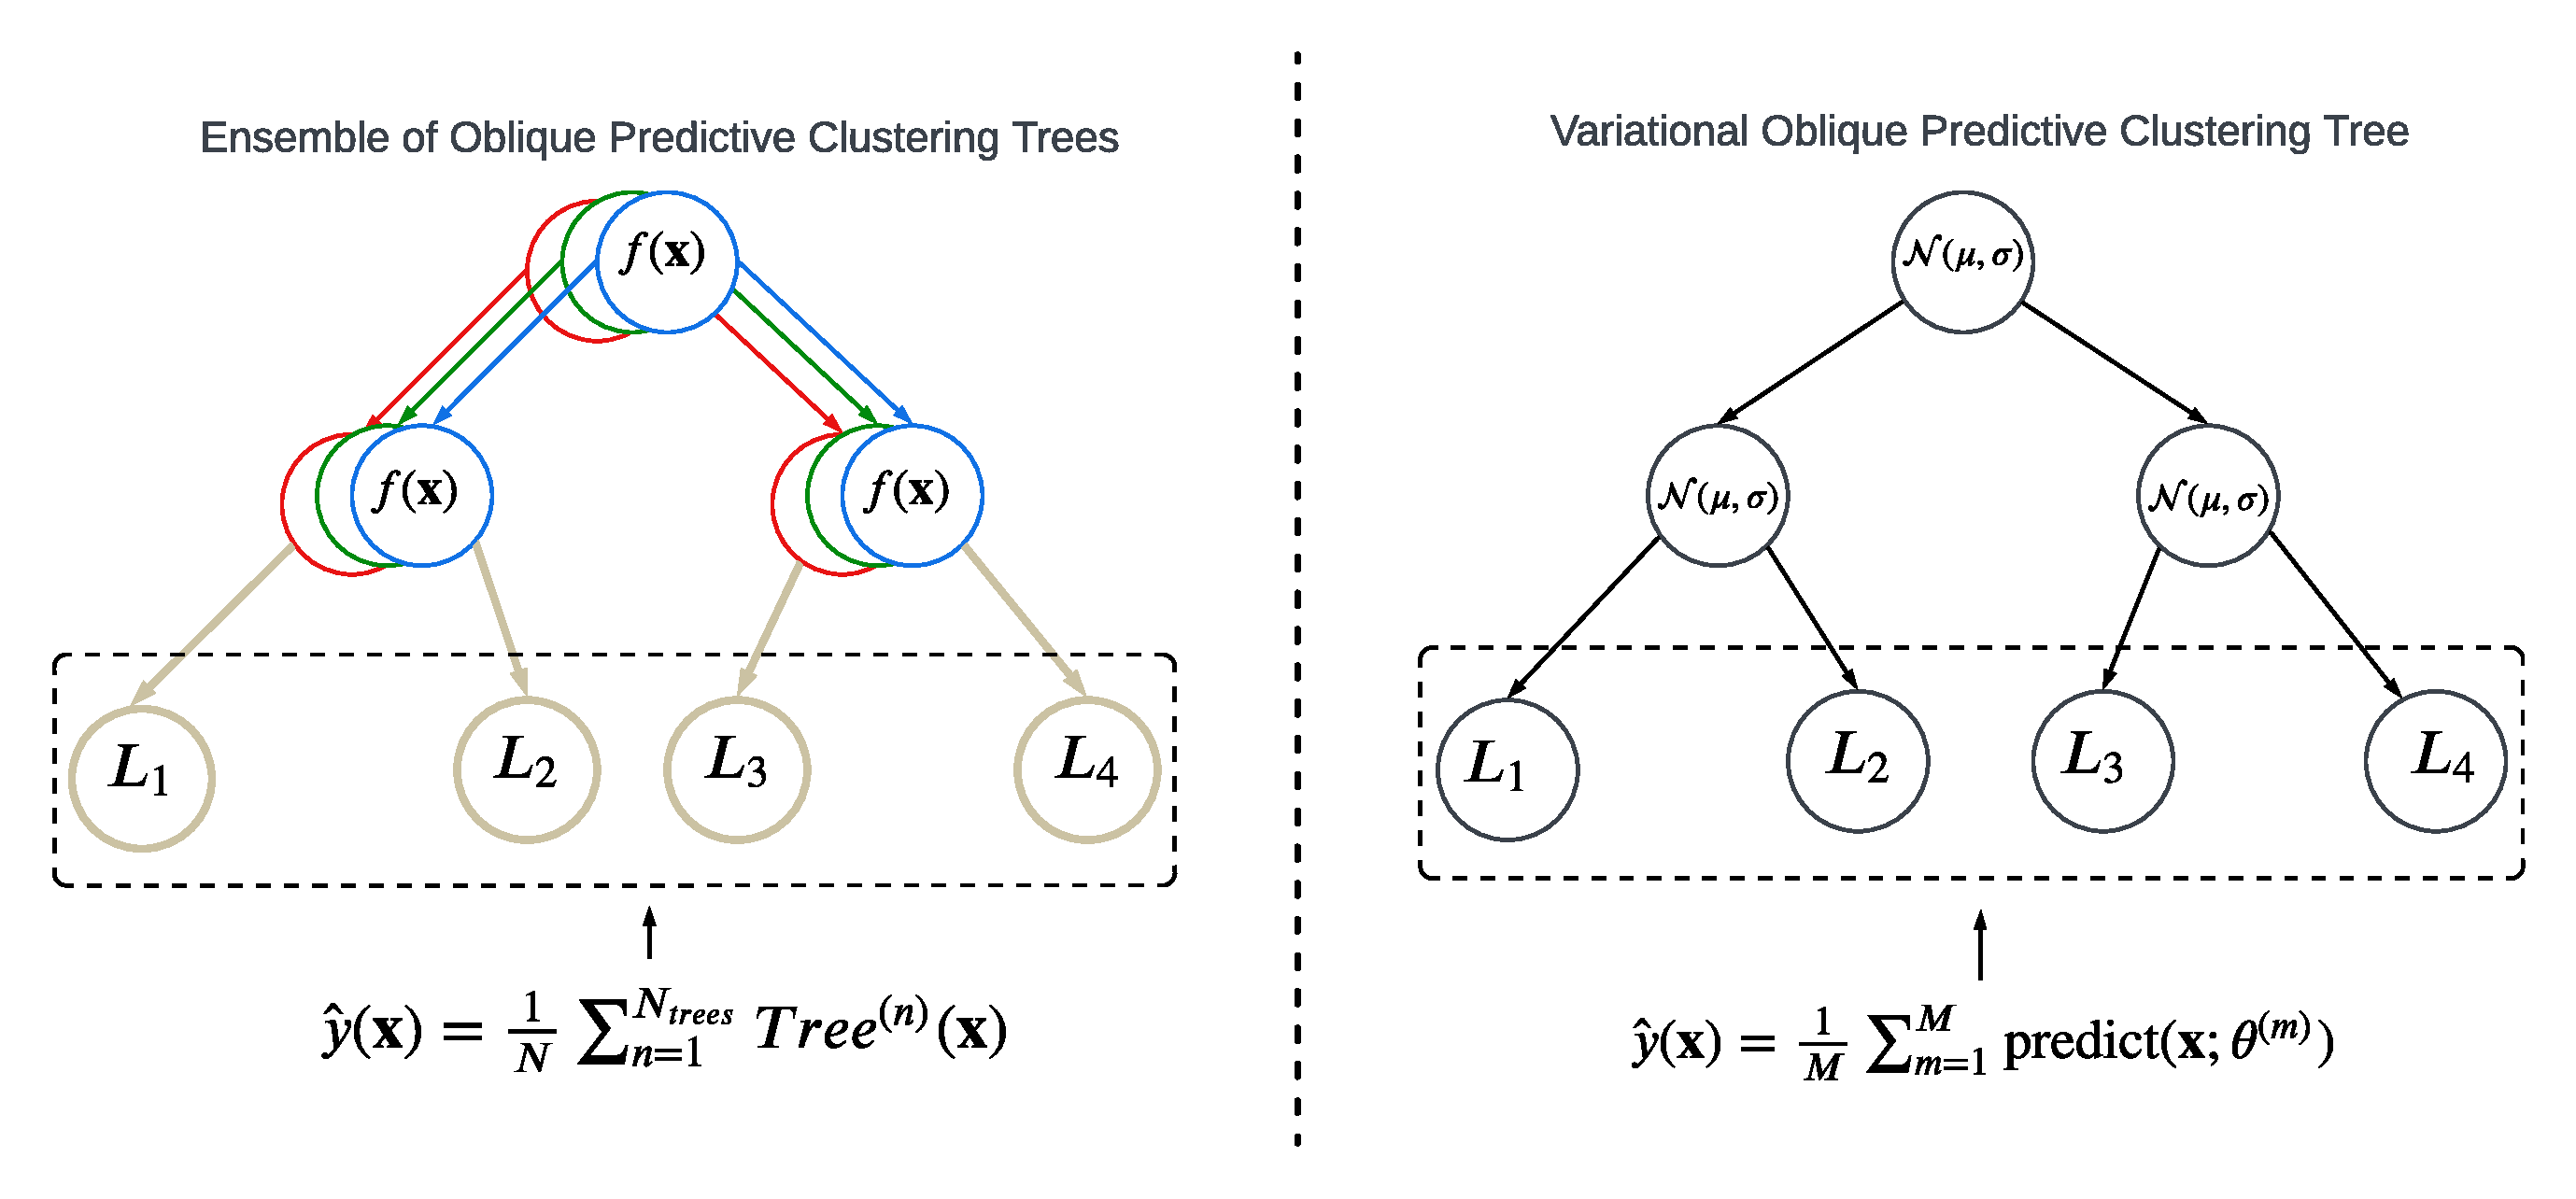
\includegraphics[width=1.0\textwidth]{main_flowchart.pdf}
    \caption{Ensemble of trees vs. Variational tree}
    \label{fig:main_flowchart}
\end{figure}

Our proposed \gls{vspyct} framework diverges from traditional ensemble approaches by directly incorporating Bayesian principles into oblique decision trees' architecture.
This model avoids conventional ensemble strategies, which aggregate multiple trees' outputs, for a probabilistic treatment of model parameters, offering refined mechanisms for uncertainty quantification and predictive performance.
The core of \gls{vspyct}'s innovation lies in applying the variational Bayes method for optimising parameters defining the oblique splits, modelling these parameters as random variables with Gaussian distributions.
This represents a paradigm shift toward a probabilistic understanding of decision-making processes within tree-based models, significantly enhancing interpretability, especially in uncertainty estimation domains.
The whole framework is given in Figure~\ref{fig:flowchart}

\begin{figure}[h!]
    \centering
    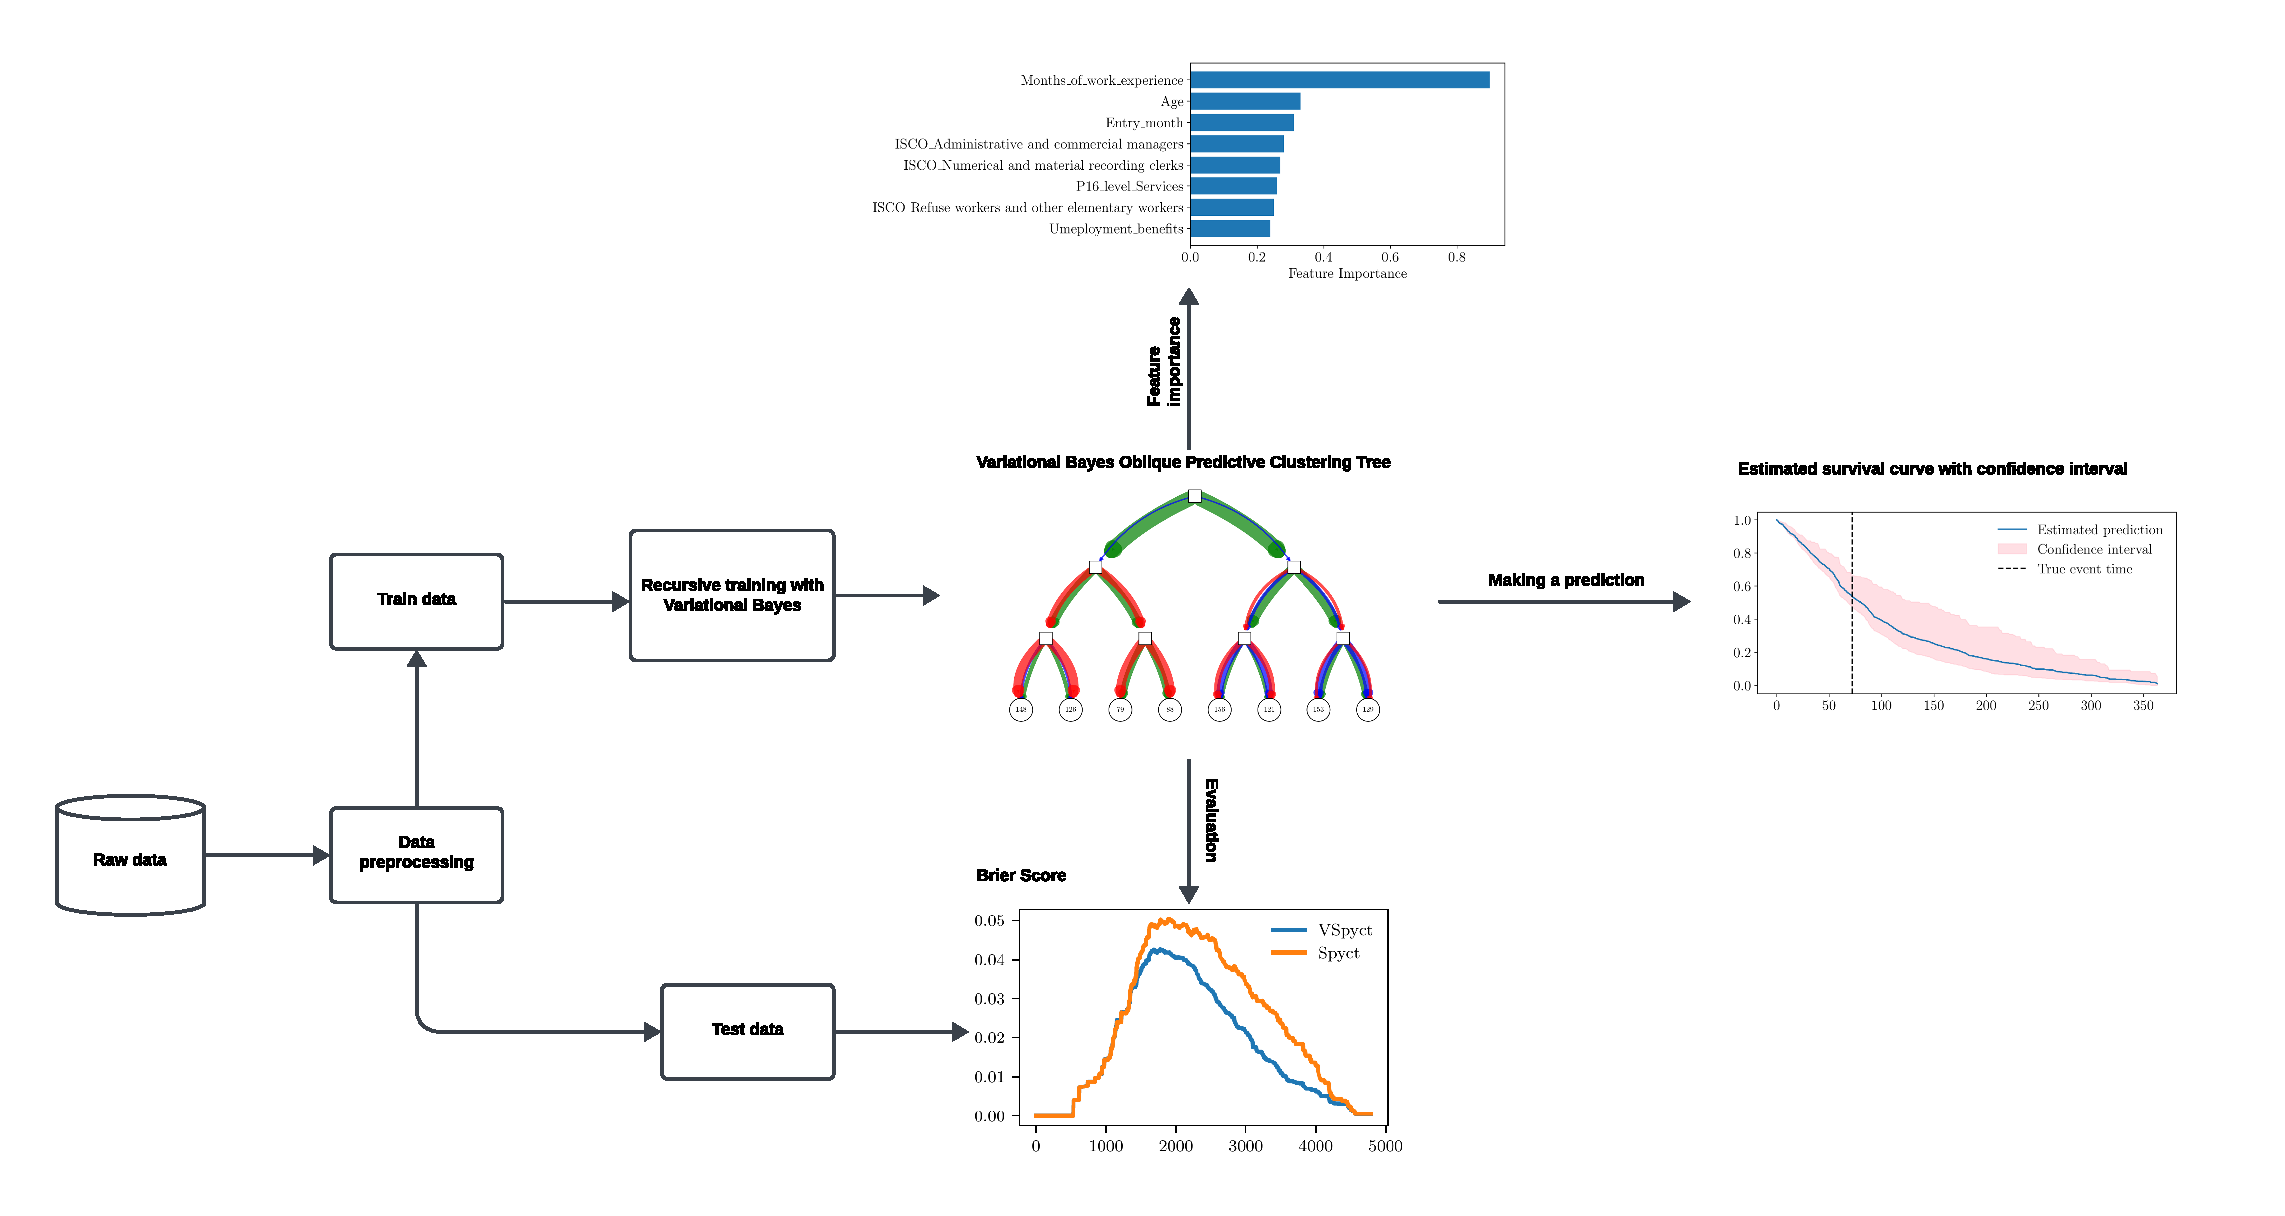
\includegraphics[width=1.0\textwidth]{methodology_flowchart.pdf}
    \caption{Flowchart of the methodology}
    \label{fig:flowchart}
\end{figure}

It sets a new benchmark for interpretable, efficient, and reliable machine learning models.

%citiraj community detection (nasiot trud), rise of gen-ai/black-box ai/llms (llama, bert, gpt), post-hoc explainability (shap),  vb metodot, 

\section{Related work}

%references for VB applications in ML and Survival analysis models. Cite pavles paper.

\Glspl{pct} have been an essential development in extending decision tree capabilities to a variety of predictive modelling tasks, including structured output prediction.
\Glspl{pct} are versatile and can be combined into ensembles to achieve state-of-the-art performance~\citep{Kocev_2013}.
However, as the dimensionality of the output space increases, the learning time of \glspl{pct} scales poorly, posing challenges in tasks like hierarchical multi-label classification where outputs can consist of hundreds of potential labels.

\Glspl{pct} are celebrated for their interpretability and efficiency, yet they often fall short in predictive performance due to their myopic, greedy nature of selecting splits.
The introduction of option predictive clustering trees (OPCTs)~\citep{Stepisnik_2020} aimed to address this limitation by incorporating multiple alternative splits within option nodes.
This approach mitigates the inherent myopia and achieves competitive performance with ensemble methods like bagging and random forests, while still maintaining a degree of interpretability.
OPCTs, despite mitigating myopia and enhancing performance, still face challenges in maintaining interpretability when extended to complex tasks.

On the other hand, \glspl{spyct}~\citep{Stepi_nik_2021} utilise oblique splits that incorporate linear combinations of features, allowing splits to correspond to arbitrary hyperplanes in the input space.
This makes \glspl{spyct} highly efficient for high-dimensional data and capable of leveraging data sparsity.
Experimental evaluations on numerous benchmark datasets have shown that \glspl{spyct} achieve performance on par with state-of-the-art methods while being significantly faster than standard \glspl{pct}~\citep{Andonovikj_2024}.
%Moreover, meaningful feature importance scores can be extracted from SPYCT models, enhancing their interpretability.

Despite these advancements, ensemble models such as random forests and gradient boosting machines remain popular due to their superior predictive accuracy.
However, their complexity often obscures interpretability, making it challenging for users to understand the model’s decision-making process.
Efforts to bridge this gap include the iForest visual analytics system~\citep{Zhao_2019}, which summarises decision paths and tree structures within random forests, thereby making the ensemble's decisions more transparent.
Additionally, the Tree Space Prototypes approach~\citep{Tan_2020} uses representative points (prototypes) for each class, offering a more intuitive understanding of ensemble classifiers compared to traditional feature-based explanations.
Visual analytics systems like iForest and prototype-based approaches offer some clarity but do not fully resolve the complexity issue.

In critical applications, such as medical diagnosis, the need for transparent and trustworthy predictions is paramount.
Methods for explaining classifier predictions and estimating the reliability of regression predictions, as demonstrated in breast cancer recurrence prediction, provide users with additional insights and build trust by clarifying the decision-making process.
Similarly, the MAPLE~\citep{plumb2018model} model combines local linear modelling with a dual interpretation of random forests, offering faithful self-explanations and maintaining high predictive accuracy.
MAPLE addresses the accuracy-interpretability trade-off and provides both example-based and local explanations, making it a comprehensive tool for understanding model behaviour.
Methods like MAPLE and other interpretability frameworks strike a balance between accuracy and transparency, but they often fall short in handling high-dimensional, sparse data efficiently.

While significant progress has been made in improving decision tree models and their ensembles, several weaknesses remain.
Many of these approaches lack inherent mechanisms for uncertainty quantification, which is crucial for applications requiring high reliability and decision certainty.

Our proposed \glspl{vspyct} model addresses these critical challenges by integrating Bayesian principles directly into the decision tree framework.
%Unlike traditional ensemble strategies, \glspl{vspyct} employs a probabilistic treatment of model parameters through the variational Bayes method, which enhances interpretability and provides inherent uncertainty quantification.
This approach maintains the clarity and simplicity of a single tree model while achieving state-of-the-art performance, thus offering a significant improvement over existing methods.
By introducing uncertainty quantification directly into the decision-making process, \glspl{vspyct} enhances the reliability and applicability of the model across various domains where decision certainty is crucial.
%This advancement bridges the gap between theoretical developments and practical applications, marking a significant step forward in making complex decision trees more accessible, interpretable, and effective.


\section{Preliminaries}

\subsection{Variational Bayes method}

% optional slika - Optimisation process of finding the closest variational distribution qω(θ) over the set of latent variables ω. (da se generira vo python)

In conducting a stochastic analysis, like survival analysis, the process of inferring model parameters hinges on applying Bayes' theorem.
For observations $x$ produced by a system defined by parameters $\theta$, Bayes' theorem is given as:

\begin{equation}
p(\theta|x)=\frac{p(x|\theta)p(\theta)}{p(x)}
\label{eq:bayes_rule}
\end{equation}

Here, the model-prescribed likelihood $p(x|\theta)$ and the selected prior $p(\theta)$ are generally well-defined.
The primary computational challenge arises in determining the posterior distribution $p(\theta|x)$ due to the denominator $p(x)$, which is derived as:

\begin{equation}
p(x)=\int_{\theta} p(x|\theta)p(\theta) \,dx,
\label{eq:evidence}
\end{equation}

This integral rarely yields a closed-form solution.
For cases with multiple dimensions, the computational burden often renders Monte Carlo methods infeasible.
The VB approach offers an approximation to this issue by closely mimicking the true posterior $p(\theta|x)$ with an approximate distribution $q_{\omega^*}(\theta)$. This variational distribution is part of a family of distributions $q_\omega(\theta)\in \mathcal{Q}$, parameterized by $\omega \in \Omega$, where $\Omega$ represents the potential latent parameter values.
Typically, the mean-field variational family is utilized, assuming independence among the parameters $\omega$\pbnote{Add citation}. 
To find the optimal $\omega^*$, one minimises the Kullback–Leibler (KL)\pbnote{Use glossaries} divergence $KL(q_\omega(\theta) \parallel p(\theta|x))$:

\begin{equation}
\omega^* = \argmin_{\omega \in \Omega}KL(q_\omega(\theta) \parallel p(\theta|x))
\label{eq:optim}
\end{equation}

Given the unknown nature of the true posterior, a rearrangement is needed to compute the KL divergence, simplifying to \pbnote{mislam deka ne ti treba celiot derivation. Može da napraviš referenca do PML2 od Murphy in da go dadeš samo poslediont red}:

\begin{align*}
KL(q_\omega(\theta) \parallel p(\theta|x)) &= \mathbb{E}_q\left[\log \frac{q_\omega (\theta)}{p(\theta|x)}\right] \\
&=\mathbb{E}_q\left[\log q_\omega(\theta)\right]-\mathbb{E}_q\left[\log p(\theta|x)\right]\\
&=\mathbb{E}_q\left[\log q_\omega(\theta)\right]-\mathbb{E}_q\left[\log p(x,\theta)\right]\\
&=\mathbb{E}_q[\log q_\omega(\theta) - \log p(x,\theta)+\log p(x)]\\
&=-\mathbb{E}_q\left[\log q_\omega(\theta) - \log q_\omega(\theta)\right] + \log p(x)\\
&\quad \quad \underbrace{\phantom{\mathbb{E}_q\left[\log q_\omega(\theta) - \log q_\omega(\theta)\right]}}_{\text{ELBO}}
\label{eq:kl_divergence}
\end{align*}

Maximising the ELBO\pbnote{Use package glossaries for abbreviations} inversely minimises the KL divergence, with $\log p(x)$ remaining constant and excluded from the optimisation \pbnote{why is it excluded, explain}.
Typically, the ELBO maximisation criterion is non-convex, with no assurance of global extremum convergence by optimisation algorithms \pbnote{True, add citation}.
Various algorithms have been employed for this challenge, including coordinate ascent variational inference and stochastic variational inference~\citep{hoffman2013stochastic}, with the latter's gradient calculated as per the black-box variational inference~\citep{sashank2018convergence}.
\pbnote{Ne se samo tie. Vidi tuka \url{https://probml.github.io/pml-book/book2.html} chapter 10}
The adoption of an approximate variational distribution introduces bias \pbnote{True, but explain where the bias is} contingent on the chosen variational family $\mathcal{Q}$, necessitating a decision grounded in empirical evidence or expert knowledge.
Despite this bias, VB's computational efficiency significantly surpasses traditional methods like Monte Carlo integration.
In our work, the ADAM optimiser~\citep{kingma2014adam} is used to facilitate the ELBO optimisation.


\subsection{Semi-supervised Multi-target Regression in Survival Analysis}
\pbnote{Do we need this subsection here? Maybe put the name to methodology, 3.1. is VB and then continue directly to 4. This subsection can go into results or application and you can actually reference it from ESWA paper}
Survival analysis primarily focuses on time-to-event data, where not all events are fully observed due to some form of censoring that halts observation before the event transpires.
The most prevalent form of censoring in this context is right-censoring, which occurs when there is incomplete knowledge about the survival time at the end of the follow-up period.
As a result, each survival record is characterised by three elements: the actual survival time $T$, its observed component $t$, and a binary indicator $\delta$, which is defined as:
\begin{equation}
\delta = \begin{cases}
0, & \text{if } T>t \text{ indicating a right-censored record},\\
1, & \text{if } T=t \text{, denoting that the event has been observed and the record is not censored}.
\end{cases}
\label{eq:delta}
\end{equation}

Moreover, assume that each observation is described by a set of covariates or features $\mathbf{X}_i=\{x_{i_1},\ldots,x_{i_N}\}$.
Thus, each record $i$ comprises the variables $\mathbf{X}_i$, $t_i$, and $\delta_i$ as specified in~\eqref{eq:delta}.
If $\delta_k=1$, the event is confirmed to have occurred at time $t_k$ and $y_{k_j} = 0$ for all $j \geq{k}$.
Conversely, if $\delta_k=0$, it implies that the fate of the instance beyond time $t_k$ is unknown, making $y_{k_j}$ missing for $j \geq{t_k}$.
This scenario of censored examples introduces missing data, which makes such datasets apt for semi-supervised learning methodologies."


\section{Methodology}

As a main part of the \gls{vspyct} model lies the oblique tree structure, which is a form of a \gls{pct} where splits are made using linear combinations of the input features rather than single features.
This allows for more complex decision boundaries, capturing intricate patterns in the data with fewer nodes compared to axis-aligned trees.
However, unlike traditional oblique trees that fix the parameters of these linear combinations, \gls{vspyct} introduces a probabilistic twist: the parameters of the splits are \mpop{not single fixed values but are instead}{} modelled as random variables \pbnote*{It does not need to be Gaussian}{with Gaussian distributions}.
This probabilistic representation captures the uncertainty in the model parameters \pbnote*{Why noisy data, what if we have perfect data but wrong model}{, a feature that is particularly useful in scenarios with noisy data}.
The construction of the \gls{vspyct} \pbnote{here you can say that the consutrction follows SPYCT, because the process is the same. Only the optimisation step is different. Explain this better here}begins with a root node and iteratively expands by adding internal nodes or leaves through a learning process based on the variational Bayes method.
Each node represents a binary decision point where instances are split into two child nodes.
At each internal node, a variational Bayes approach is used to learn the parameters of an oblique split.
\pbnote*{Keep ELBO until later. Here explain the basic SPYCT, there are no stochastic parts here yet} {This involves optimising the parameters of a linear model that best divides the data to minimise the ELBO.}
The linear model is defined as:

\begin{equation}
f(\mathbf{x})=\sigma \left(\mathbf{w}^T \mathbf{x} + b \right)
\label{eq:linear_model}
\end{equation}

where $\mathbf{x} \in \mathbb{R}^N$ is the feature vector, $\mathbf{w} \in \mathbb{R}^N$ represents the weights, $b \in \mathbb{R}$ is the bias, and $\sigma(\cdot)$ denotes the sigmoid function ensuring the output lies in $(0, 1)$, indicating the probability of branching to the right child node.


\pbnote{The part below should be separate. Above explain how the mechanism of SPYCT works. Below you can point out the main difference. May be merge this with the next subsection, but it shoud le rewritten carefully.
Here you are missing your key idea. How to minimise the impurity function. You got an idea that you should put the target value at 0 and run ELBO on it. This is missing here.}
The learning process involves defining a prior distribution over the weights and biases, typically Gaussian, and updating this to a posterior distribution given the observed data through variational inference.
The ELBO is optimised using stochastic gradient descent, with the learning rate $\alpha$ and potentially variable batch sizes $B$.
The split at each node is determined by evaluating the learned linear model on the descriptive data.
Instances are split based on the probability threshold of $0.5$, with those having a probability greater than $0.5$ moving to the right child node and the rest to the left.
For leaf nodes, a prototype is computed as the mean of the target variables for the instances assigned to the leaf.
This prototype represents the prediction for instances that fall into the leaf during the prediction phase.


\subsection{Learning splits using Variational Bayes}

% optional: computation graph diagram

The learning of these Gaussian-distributed parameters is achieved through a Variational Bayes (VB) method.
In the context of \gls{vspyct}, the VB method is employed to learn the Gaussian distributions representing the parameters of the oblique splits.
The process involves defining a prior distribution over the parameters and then updating this prior to a posterior distribution given the observed data.
This is done by optimising the ELBO, which balances the fit of the model to the data with the complexity of the model.
The procedure for learning a split using the VB method is given in Algorithm~\ref{alg:learn_split}.

\begin{algorithm}[h!]
\caption{Variational Learning of Split Parameters in \gls{vspyct}}
\label{alg:learn_split}
\begin{algorithmic}[1]

\State \textbf{Input:} Dataset $\mathcal{D}$, features $\mathbf{X}$, targets $\mathbf{Y}$, parameters $\theta$, epochs $E$, batch size $\beta$, learning rate $\lambda$, selection probability $\sigma$
\State \textbf{Output:} Parameters $\Theta$, guide $\mathcal{G}$

\Procedure{LearnSplit}{$\mathcal{D}$, $\mathbf{X}$, $\mathbf{Y}$, $\theta$, $E$, $\lambda$, $\beta$, $\sigma$}
    \State $\Phi \sim \text{Bernoulli}(\sigma)$ \Comment{Select attributes based on probability $\sigma$}
    \State $\mathbf{X}_\Phi \leftarrow$ subset of $\mathbf{X}$ using $\Phi$
    \State Model $\mathcal{M} \leftarrow \text{Define Impurity}(\dim(\mathbf{X}_\Phi), 1, \theta)$
    \State Guide $\mathcal{G} \leftarrow \text{Define AutoDiagonalNormal}(\mathcal{M})$
    \State Define optimization parameters $\alpha \leftarrow \{\text{"lr"}: \lambda\}$
    \State Initialise optimizer $\text{Optimizer} \leftarrow \text{Adam}(\alpha)$
    \State Early stopping mechanism $\text{EarlyStopping} \leftarrow \text{Initialize}(\beta)$
    
    \State Initialise loss list $L$
    \State Calculate number of batches $B \leftarrow \lceil \frac{|\mathcal{D}|}{\beta} \rceil$
    
    \For{$e \in \{1, \dots, E\}$}
        \State Initialise training loss $\mathcal{L}_{\text{train}} \leftarrow 0$
        \For{$b \in \{1, \dots, B\}$}
            \State $(\mathbf{X}_b, \mathbf{Y}_b) \leftarrow \text{Get Batch}(\mathbf{X}_\Phi, \mathbf{Y}, b, \beta)$
            \State Update training loss $\mathcal{L}_{\text{train}} \leftarrow \mathcal{L}_{\text{train}} + \text{SVI Step}(\mathcal{M}, \mathcal{G}, \mathbf{X}_b, \mathbf{Y}_b)$
        \EndFor
        \State Append $\mathcal{L}_{\text{train}}$ to $L$
        \If{$\text{EarlyStopping}(\mathcal{L}_{\text{train}})$}
            \State \textbf{break}
        \EndIf
    \EndFor
    \State \Return $\mathcal{M}$, $\mathcal{G}$
\EndProcedure

\end{algorithmic}
\end{algorithm}

\pbnote{Algorithm Impurity is not referenced anywhere in the text. Do you need it at all?}
\begin{algorithm}[h!]
\caption{Impurity}
\begin{algorithmic}[1]

\Procedure{Impurity}{$\xi$, $\zeta$, $\theta$}
    \State $\mathbf{w}, b \sim \mathcal{N}(0, I)$ \Comment{Weight and bias priors}
    \State $\rho(\mathbf{x}) \gets \sigma(\mathbf{w}^\top \mathbf{x} + b)$ \Comment{Right selection probability}
    \State $\lambda(\mathbf{x}) \gets 1 - \rho(\mathbf{x})$ \Comment{Left selection probability}
    \State Compute $\text{Var}_\rho(\mathbf{Y})$ and $\text{Var}_\lambda(\mathbf{Y})$ \Comment{Weighted variances}
    \State $\Omega \gets \lambda \cdot \text{Var}_\lambda(\mathbf{Y}) + \rho \cdot \text{Var}_\rho(\mathbf{Y}) + \|\mathbf{w}\|_{0.5}$
%    \State Observe $\Omega$ with likelihood $\mathcal{N}(0, 1)$
    \State \textbf{return} $\Omega$
\EndProcedure

\end{algorithmic}
\end{algorithm}

\subsection{Making a prediction}

The procedure for making a prediction for a new instance using the \gls{vspyct} model is given in Algorithm~\ref{alg:make_pred}.
\pbnote{How? What do you get from predictive? Why do you need predictive, why not just using the estimated model parameters directly? This subsection is not written OK!} 
\pbnote{What is prototype in Algorithm~\ref{alg:make_pred}?} 
\pbnote{Can you write this in a mathematical form}
It involves traversing the tree from the root to a leaf, at each internal node using the variational posterior to sample parameters and compute the probability of branching right or left.
The prediction of the reached leaf's prototype is returned as the output.
Operationally, when a new data point is to be classified or a prediction is to be made, it traverses the tree from the root to a leaf.
At each node, the oblique split is determined by evaluating the linear combination of the input features, with parameters sampled from the learned Gaussian distributions.
This probabilistic approach to decision-making within the tree allows for a more nuanced interpretation of the data, accounting for uncertainty in the model parameters.

\begin{algorithm}
\caption{\gls{vspyct} Prediction Process}
\label{alg:make_pred}
\begin{algorithmic}[1]

\State \textbf{Input:} Feature vector $\mathbf{x}$, decision tree $T$ rooted at node $\Omega$
\State \textbf{Output:} Prediction $\hat{y}$

\Function{Predict}{$\Omega$, $\mathbf{x}$}
    \If{$\Omega$ is a leaf}
        \State \Return $\Omega.prototype$
    \Else
        \State $\Theta \gets$ \Call{SampleParameters}{$\Omega.split\_model$, $\Omega.guide$}
        \State Define sigmoid function $\rho(\Theta, \mathbf{x}) = \frac{1}{1 + \exp(-\Theta^\top \mathbf{x})}$
        \If{$\rho(\Theta, \mathbf{x}) \leq 0.5$}
            \State \Return \Call{Predict}{$\Omega.left$, $\mathbf{x}$}
        \Else
            \State \Return \Call{Predict}{$\Omega.right$, $\mathbf{x}$}
        \EndIf
    \EndIf
\EndFunction

\Function{SampleParameters}{model, guide}
    \State Let $\Theta = (\mathbf{w}, b)$ where:
    \State $\mathbf{w}$ are weights sampled from variational posterior $q_{\omega}(\mathbf{w}|\mathcal{D})$
    \State $b$ is bias sampled from variational posterior $q_{\omega}(b|\mathcal{D})$
    \State \Return $\Theta$
\EndFunction

\State Compute prediction $\hat{y}$ by invoking \Call{Predict}{$\Omega$, $\mathbf{x}$}
\State \textbf{Return} $\hat{y}$

\end{algorithmic}
\end{algorithm}


\subsection{Time complexity analysis}

In this section, we analyse the time complexity of learning a split in \gls{vspyct} and compare it with \gls{spyct}.
Our analysis focuses on the computational expense associated with determining a split, as this represents the principal distinction between the two approaches.
In the predictive clustering framework, the set of clustering attributes $K$, which contributes to the variance calculation, encompasses both the features and the target variables.
As a result, $K$ equals $N + T$, with $N$ representing the feature count and $T$ denoting the target count.
The time complexity for learning in \glspl{spyct} can be expressed as $\mathcal{O}(NI_o(D+K))$, wherein $I_o$ stands for the iteration count needed for optimisation\pbnote{Citation}.
Notably, the computational demand for the \glspl{spyct}' gradient-based version increases linearly with the attribute count.

The introduction of variational Bayes method in the architecture of \gls{spyct} to create \gls{vspyct} adds a new layer of computational complexity.
Specifically, the variational approach requires iterating over the dataset multiple times to optimise the ELBO for each split.
This iterative process involves sampling from the posterior distributions of split parameters, evaluating the ELBO, and updating the parameters accordingly.
Consequently, the time complexity for learning a split in \gls{vspyct} can be described as $\mathcal{O}(MI_oNI_{vb})$, where $M$ is the number of Monte Carlo samples used to approximate the posterior distributions, $I_{vb}$ represents the number of iterations required for variational inference to converge, and the other variables retain their meanings from the \gls{spyct} context \pbnote{This is great but you have to explain how did you get to this complexity. Can you write the derivation}.

Comparing \glspl{vspyct} to \glspl{spyct}, the introduction of variational Bayes method increases the computational load due to the necessity of Monte Carlo sampling and iterative ELBO optimisation.
However, this additional complexity is counterbalanced by the enhanced predictive performance, model interpretability, and uncertainty quantification offered by \glspl{vspyct}.
%While \glspl{spyct} are computationally efficient due to their linear scaling with the number of attributes and utilisation of gradient-based optimisation, \glspl{vspyct} leverage the power of variational inference to provide a deeper understanding of the data and model behaviour, even if at the cost of increased time complexity.

\pbnote{Maybe this paragraph can go to conclusion or discussion}
The choice between using \glspl{vspyct} over \glspl{spyct} hinges on the specific requirements of the application scenario.
For tasks where model interpretability and uncertainty quantification are paramount, and computational resources are sufficient, \glspl{vspyct} offer a compelling advantage.
Conversely, for applications where computational efficiency is critical, and the interpretability requirements are less stringent, \glspl{spyct} may still be favourable.

\subsection{Feature importance}

\pbnote*{Complex sentence}{Feature importance is derived from the aggregated impact of features across all splits, quantified by examining the variational posterior distributions of the weights.}
The importance of each feature is proportional to its contribution to reducing impurity across splits.

Given a \gls{vspyct} model, the feature importances are derived from the variational parameters defining the split decisions across the tree.
The essence of the computation lies in evaluating the expected influence of each feature, taking into account the probabilistic nature of the model parameters.
This is encapsulated by the following formula:

\begin{equation}
\text{Imp}(T) = \sum_{s \in T} \left( \frac{s_n}{N} \right) \left( \frac{\mathbb{E}[\mathbf{w}_s]}{|\mathbb{E}[\mathbf{w}_s]|_1} \right)
\end{equation}
where $s$ is a split in the variational oblique predictive clustering tree $T$, $s_n$ is the number of training examples that passed through node $s$, \pbnote*{Shoudn't this be $N_s$}{$N$} denotes the total number of training examples used in the tree, $\mathbf{w}_s$ symbolizes the weight vector defining the oblique split at node $s$\mpop{, treated as a random variable with a Gaussian distribution}{}, $\mathbb{E}[\mathbf{w}_s]$ signifies the expected value \mpop{(mean)}{ }of the weight vector $\mathbf{w}_s$, calculated from its \pbnote*{Careful, posterior or vairational or predictive}{posterior} distribution as inferred by the variational Bayesian method.
The normalization factor \pbnote*{What does $_1$ mean? Can you give a complete definition}{$|\mathbb{E}[\mathbf{w}_s]|_1$} ensures the comparability of feature importances by scaling them relative to the aggregate magnitude of expected weights.
This formulation accounts for the stochastic nature of each parameter, reflecting the central tendency of the distributions defining the split hyperplanes.

For practical computation, the expected weights $\mathbb{E}[\mathbf{w}_s]$ are obtained by sampling from the \pbnote*{Again which? Where in the code is this?}{posterior} distributions inferred during the learning process.
Each weight vector $\mathbf{w}_s$ is drawn such that $\mathbf{w}_s \sim q(\mathbf{w}_s|\mathcal{D})$, where $q(\mathbf{w}_s|\mathcal{D})$ represents the \pbnote*{so, variational approximation not the posterior}{variational approximation} to the posterior distribution of weights given the data $\mathcal{D}$.
The importance of each feature is then a function of these expected weights, modulated by the frequency of training instances influencing each split, thereby emphasising the splits that impact a larger portion of the data.
This mathematical framework for computing feature importances in \gls{vspyct} not only highlights the contribution of individual features to the model's decision-making process but also integrates the inherent uncertainty of these contributions, offering a richer, more nuanced understanding of feature relevance within a probabilistic modelling context.

\pbnote{This is rather complex subsection it needs more bachground. How did you come up with the idea of this relation, provide simple toy example with 2 or 3 weights to explain how this works}


\section{Data and evaluation metric}
\pbnote{Now I understand. Why did you focus only on survival data. If I remember correctly you calculated the performance on different data sets not just survival. If we leave it only on this it will not go OK with the review.}

\subsection{Data}

\subsection{R Survival datasets}

Our evaluation encompasses four benchmark survival analysis datasets, each serving as a standard reference within the domain and accessible via the survival R package~\citep{survival-package}.

\begin{enumerate}
\item \textit{Retinopathy Dataset}: Investigates the efficacy of laser coagulation in delaying vision loss due to diabetic retinopathy among 197 patients, with survival times adjusted for a minimum event horizon of 6.5 months.
\item \textit{Lung Dataset}: Analyses survival data for patients with advanced lung cancer, focusing on their lifespan post-diagnosis and daily activity performance levels.
\item \textit{Primary Biliary Cirrhosis (PBC) Dataset}: Examines the progression of primary biliary cholangitis in 424 patients, with data drawn from a clinical trial conducted between 1974 and 1984, exploring disease progression towards cirrhosis.
\item \textit{Heart Dataset}: Studies the survival of patients on the waiting list for heart transplants at Stanford, evaluating the length of time patients remain on the waiting list.
\end{enumerate}

\begin{table}[h!]
\centering
\caption{Main properties of the datasets. Censoring shows the percentage of censored observations.}
\adjustbox{max width=\textwidth}{
\begin{tabular}{llll}
\toprule
Dataset& \# of examples& \# of features& Censoring\\
\midrule
Mayo Clinic Primary Biliary Cholangitis&312&17&60\%\\
NCCTG Lung Cancer&228&8&\\
Stanford Heart Transplant&172&4&\\
Retinopathy&394&9&\\
\bottomrule
\end{tabular}
}
\label{table:dataset}
\end{table}%



\subsection{Unemployment dataset}
The dataset we consider consists of $74,086$ instances and contains anonymised personal and professional characteristics of jobseekers that have entered the Slovenian \gls{pes}.
The dataset is complex because its attributes come in different forms (categorical, numerical, date and time), and most have to undergo transformation.
An overview of the dataset and its features is given in \tablename~\ref{table:dataset}.

\begin{table}[h!]
\centering
\caption{Features of the dataset and their cardinalities \citep{Andonovikj_2024}}
\begin{tabular}{ll}
\toprule
Continuous features& Discrete features\\
\midrule
Day of PES entry&Education direction (30)\\
Months of work experience&Occupation (ISCO) (123)\\
Age&Reason for PES entry (5)\\
Month of PES entry&Reason for termination (43)\\
&Social benefits (2)\\
&Gender (2)\\
&eApplication (2)\\
&Unemployment benefits (2)\\
\bottomrule
\end{tabular}
\label{table:dataset}
\end{table}%

The general structure of the jobseekers' attributes is described by dividing the attributes into several prominent groups: socioeconomic variables (gender, age), information on job readiness (education, health limitations), and opportunities (regional labour market development), and all available labour market history information, such as prior work experience.
The target variable is in numeric form.
It is a counter of days till a jobseeker gets employed or gets out of the study and leaves no further information about the jobseeker's employment status.

\figurename~\ref{fig:grid_prob} shows the distributions of some features in the dataset.
The sample of jobseekers is balanced in terms of gender.
Most jobseekers enter the \gls{pes} without any working experience. 
As expected, the age distribution is between 18 and 64 since this is the legal age interval of the labour-active population.
It should be noted that the age distribution is bi-modal.
The first peak is around 23-26 years since this is the expected graduation age for a university degree.
The second peak is just before 60 years of age, i.e. jobseekers who became unemployed just before retirement due to various reasons.
The final histogram shows that the dataset contains 30\% of right censored data.

\begin{figure}[h!]
    \centering
    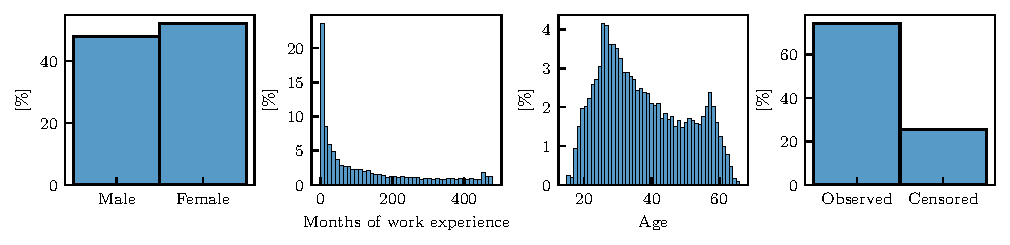
\includegraphics[width=0.95\textwidth]{feature_distributions.pdf}
    \caption{Distributions of some of the dataset features \citep{Andonovikj_2024}}
    \label{fig:grid_prob}
\end{figure}


The categorical features are diverse with respect to their cardinality.
The categories of the features with high cardinality ($>1000$ different class values per feature) are transformed using domain knowledge and the number of class values is significantly reduced.
Because the \emph{ISCO} standard and \emph{Education direction} provide a hierarchical classification of occupations and education directions, we took the higher-level classifications and thus significantly reduced the number of categories.
The remaining categorical features were encoded using one-hot encoding.
The temporal (cyclical) features, such as ``Day of PES entry" and ``Month of PES entry" were transformed by calculating the feature's $\sin$ and $\cos$ components.
In this way, the artificially significant difference between, for example, the last day of the previous month and the first day of the current month is removed, and the value of the feature can be viewed as a point $\left(\sin(x), \cos(x)\right)$ of a circle.

\subsection{Evaluation metric}

The efficacy of survival models is predominantly assessed through the Concordance Index~\citep{brentnall2018use} and the Brier score~\citep{gerds2006consistent}.
While the Concordance Index offers valuable insights, its inability to account for the error magnitude in predicted probabilities limits its utility.
The Brier score addresses this gap by factoring in the error magnitude, making it a more comprehensive metric for our experimental evaluation.
The Brier score assesses the precision of a forecasted survival function at a specific time $t$, quantifying the mean squared differences between observed survival statuses and forecasted survival probabilities.
It ranges from $0$ to $1$, where a score of $0$ indicates perfect accuracy.
This metric not only assesses the precision of time-to-event forecasts, akin to a squared error loss, but also necessitates adjustments for right-censored samples in the dataset.
This adjustment employs the inverse probability of censoring weights method to weight the squared differences.

The conditional survival function estimator for censoring times, $\hat{G}(t)=P(C>t)$, utilises the Kaplan-Meier method, with $C$ denoting the censoring time.
The Brier score is thus calculated as~\citep{trickbrier}:

\begin{equation}
BS(t) = \frac{1}{M}\sum\limits_{i=1}^N \left(\frac{\hat{S}(t_i,\mathbf{X}i)\cdot1{T_i\geq{t},\delta_i=1}}{\hat{G}({T_i}^-)}+\frac{(1-\hat{S}(t_i,\mathbf{X}i))\cdot1{T_i>t, \delta_i=0}}{\hat{G}(T_i)}\right)
\label{eq:bs}
\end{equation}

Here, $M$ signifies the count of test instances, $\mathbf{X}_i$ the feature vector for each instance, $\hat{S}(t, \mathbf{X}_i)$ the predicted survival probability at time $t_i$, $\delta_i$ a boolean indicator, and $T_i$ and $T_i^-$ the survival times for $\delta_i$ being 0 and 1, respectively. The Brier score is computed at various timestamps to evaluate how the method's performance varies with predictions extended into the future.

The performance was estimated by using $k$-fold cross-validation with the parameter $k$ set to 5~\citep{elstatl}.
The prediction model yields an estimated survival curve for each individual in the study.

\section{Results}

The resulting BS curves are shown in Figure~\ref{fig:brier_scores}.
It should be noted that lower BS indicates a more accurate forecast.
The analysis revealed distinct performance patterns between the two models across different datasets.
Specifically, in the PBC and lung cancer datasets, \gls{vspyct} outperformed \gls{spyct}, evidenced by consistently lower Brier scores throughout the observation period.
This superior performance of \gls{vspyct} could be attributed to its robust handling of parameter uncertainty through the VB method, which likely improved its predictive accuracy in these contexts.
The \gls{vspyct} model demonstrated a particularly notable advantage in maintaining lower peak Brier scores, suggesting enhanced reliability in predicting survival outcomes for patients with PBC and lung cancer.

Conversely, in the heart transplant and retinopathy datasets, \gls{spyct} showed better performance compared to \gls{vspyct}, as indicated by lower Brier scores over time.
This suggests that the simpler, more direct approach of \gls{spyct} may be more effective in certain contexts, possibly due to less complex data structures or the nature of the underlying survival processes in these specific conditions.
The lower Brier scores achieved by \gls{spyct} in these cases highlight its efficiency in accurately predicting the survival outcomes of heart transplant patients and those undergoing treatment for diabetic retinopathy.

% average rank diagram - zemi go kodot od Matej Petkovic

\begin{figure}[h!]
\centering
\subfloat[Lung]{%
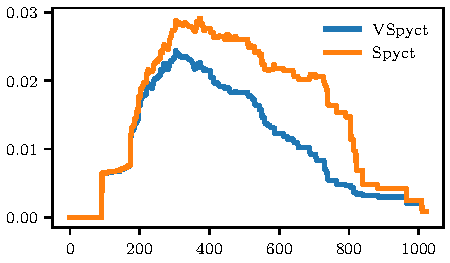
\includegraphics{bs_r_cancer.pdf}
\label{fig:bs_cancer}}
\quad % Adds some space between the figures in the same row
\subfloat[Retinopathy]{%
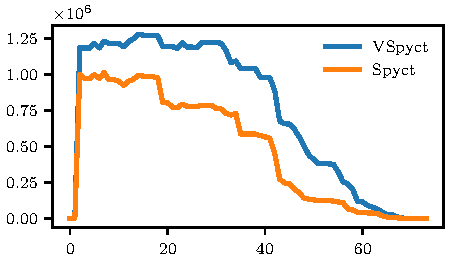
\includegraphics{bs_r_retinopathy.pdf}
\label{fig:bs_retinopathy}}\\ % Ends the first row and starts a new one
\subfloat[Heart]{%
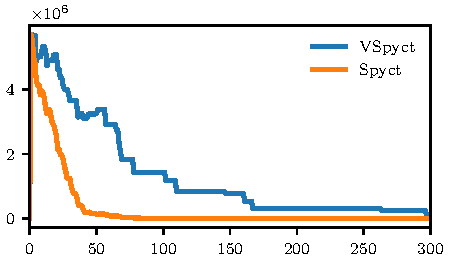
\includegraphics{bs_r_heart_truncated.pdf}
\label{fig:bs_heart}}
\quad % Adds some space between the figures in the same row
\subfloat[PBC]{%
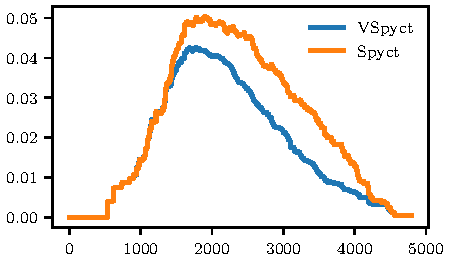
\includegraphics{bs_r_pbc.pdf}
\label{fig:bs_pbc}}

\caption{Performance evaluation of \gls{vspyct} and \gls{spyct} models measured through the Brier score on the R survival datasets}
\label{fig:brier_scores}
\end{figure}


\subsection{Interpretability}

%slika od drvoto so oboeni edges

Figure~\ref{fig:inter_tree} presents the visual representation of the \gls{vspyct} applied to the Unemployment dataset.
Based on that, one can distill a concise interpretation enriched with practical insights.

\begin{figure}[h!]
    \centering
    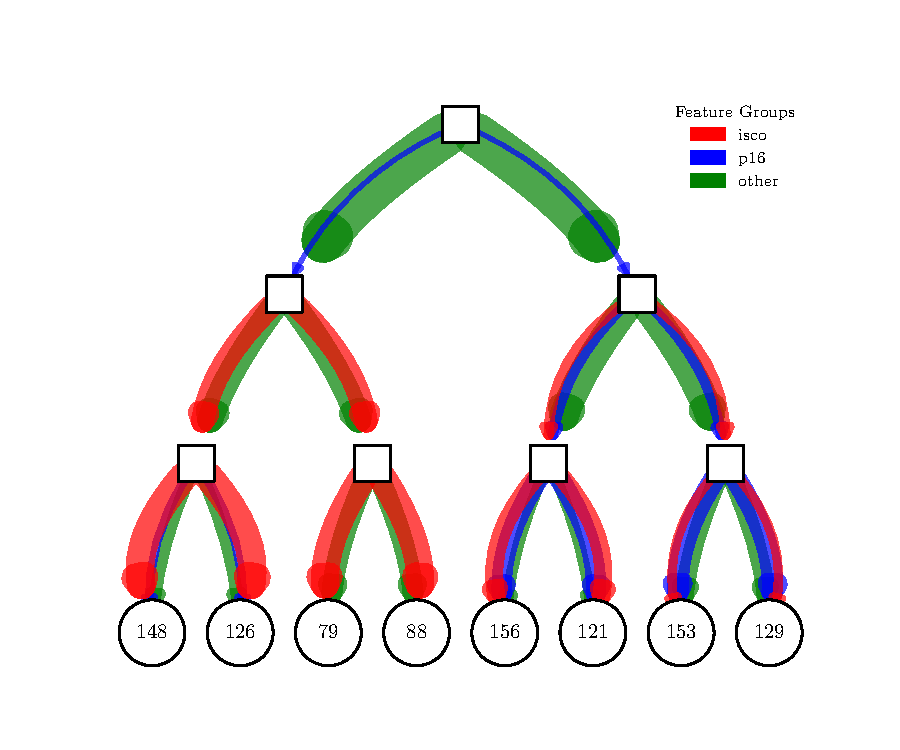
\includegraphics{hecat_tree_old_temp.pdf}
    \caption{The \gls{vspyct} model applied to the Unemployment dataset. The colouring distinguishes the different feature groups of the data set}
    \label{fig:inter_tree}
\end{figure}

At the heart of this \gls{vspyct} model lies the ability to visually demarcate the influence of various feature categories on unemployment duration predictions.
The tree's root node is predominantly influenced by features categorised under ``other" (represented in green), encompassing age, months of work experience, and various demographic characteristics.
This indicates that such features play a pivotal role in initial split decisions, underscoring the broad impact of demographic and experiential factors on unemployment trends.

As we navigate through the tree, a dichotomy emerges based on the expected survival times—essentially, the projected duration an individual is likely to remain unemployed.
On branches leading to higher expected survival times, features categorised under ``p16 level of education" (coloured in blue) become increasingly dominant.
This suggests that higher levels of education are associated with longer periods of unemployment, potentially reflecting challenges in finding employment that matches an individual's qualifications or aspirations.

Conversely, on branches associated with lower expected survival times, the dominance shifts towards features represented by the ``ISCO classification of professional occupation" (coloured in red).
This dominance implies that certain professional occupations, as defined by the ISCO classification, may expedite reemployment, possibly due to higher demand or greater flexibility in job roles within these sectors.

This visual breakdown not only highlights the model's interpretability but also offers tangible insights into how different factors—ranging from personal demographics and work experience to education and professional classifications—impact unemployment durations.
Such insights are invaluable for policymakers and stakeholders aiming to devise targeted interventions that address specific barriers to employment faced by diverse demographic groups.

In essence, the \gls{vspyct} model's tree structure, with its intuitive colour-coded feature categories and quantified predictions at the leaf nodes, offers a powerful tool for understanding the multifaceted nature of unemployment.
It bridges the gap between complex machine learning models and practical socio-economic applications, providing a clear, actionable framework for addressing unemployment through informed, data-driven strategies.

\section{Conclusion}

We introduced the \gls{vspyct} model, an approach that strategically combines the benefits of oblique splits, variational Bayes, and Bayesian inference within a single, interpretable framework.
The \gls{vspyct} model addresses the trade-off between the performance of ensemble models and the interpretability of single decision trees, and the absence of inherent uncertainty quantification in predictions.
Our results demonstrate that the \gls{vspyct} model is competitive to, and on some data sets exceeds the performance of ensemble of \glspl{spyct}, without sacrificing the model's interpretability.
By employing variational Bayes method, we introduce a mechanism for uncertainty quantification directly into the decision-making process, enhancing the reliability and applicability of the model across various domains where decision certainty is paramount.
%The \gls{vspyct} model marks a significant step forward in making complex decision trees more accessible, interpretable, and effective.
The model opens new possibilities for research in semi-supervised learning and Bayesian inference, promising to bridge the gap between theoretical advancements and practical applications.
Future work will focus on further refining the model's performance, and extending its applications in diverse \gls{sop} settings.

\section*{Acknowledgement}
The authors acknowledge the research core funding No.\ P2-0001,  P2-0103 and P2-0383 financially supported by the Slovenian Research Agency.
The authors also acknowledge the funding received from the European Union's Horizon 2020 research and innovation programme project HECAT under grant agreement No.\ 870702 .

%\printbibliography

\bibliographystyle{elsarticle-harv}
\bibliography{bibliography}

\end{document}
